\chapter{Arquitectura y Diseño}
\label{chapter:4-Arquitectura y Diseño}
En este próximo capítulo se describe la arquitectura realizada a alto nivel. En este capítulo se detalla y se explica la arquitectura final del producto. 
El capítulo se separa entre las secciones de arquitectura del frontend y backend.

\section{Arquitectura}
\label{section:4-2-Arquitectura}
La sección está divida por \gls{frontend} y \gls{backend}.

\subsection[Frontend]{Frontend}
\label{subsection:4-2-frontend}
El \gls{frontend} está compuesto por 

\begin{figure}[htbp]
    \centering
    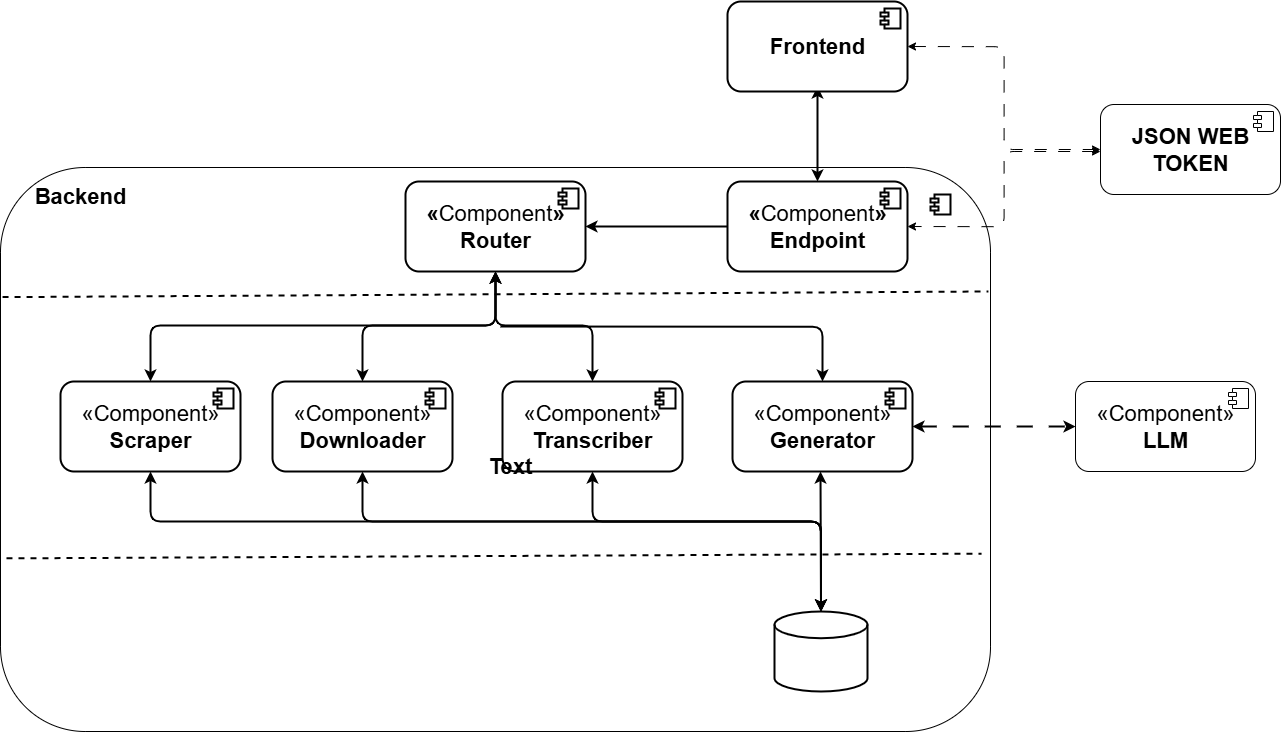
\includegraphics[width=\linewidth]{Nuestro/Imagenes/Arquitectura/Backend.drawio.png}
    
    \caption{Diagrama UML de los componentes del \gls{backend}. Ilustración propia.}
    \label{fig:Arquitectura_Backend}
\end{figure}

\begin{figure}[htbp]
    \centering
    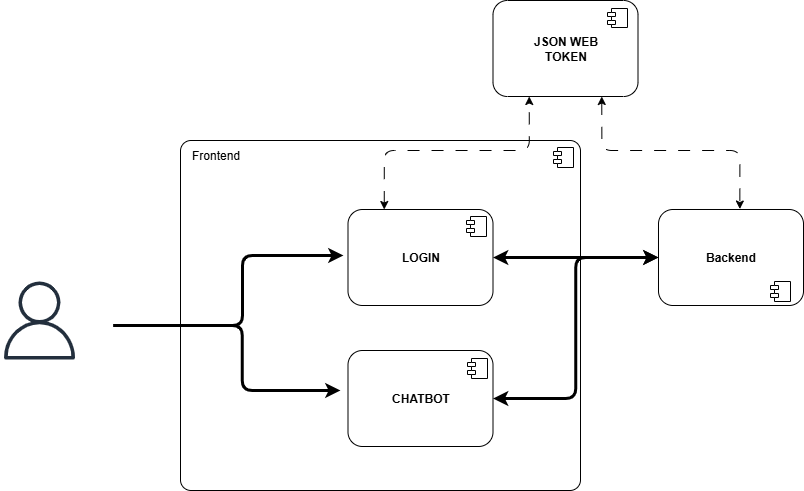
\includegraphics[width=\linewidth]{Nuestro/Imagenes/Arquitectura/Frontend.png}
    
    \caption{Diagrama UML de los componentes \gls{frontend}. Ilustración propia.}
    \label{fig:Arquitectura_Frontend}
\end{figure}



\subsection[Componentes del Backend]{Componentes del backend}
\label{subsection:4-2-Componentes del backend}

El \gls{backend} del sistema se estructura en módulos especializados que operan de forma independiente pero coordinada, siguiendo principios de arquitectura de microservicios. Cada componente tiene una responsabilidad claramente delimitada dentro del pipeline de procesamiento, desde la adquisición de contenido hasta la generación de respuestas contextualizadas. Esta separación modular facilita el mantenimiento, testing y escalabilidad del sistema. A continuación se detallan los cinco componentes principales que conforman la arquitectura \gls{backend}.
\subsection{Scrapper}
\label{subsection:5-Scrapper}

Componente encargado de la extracción automatizada de metadatos desde la plataforma \Gls{OpenFing}. Realiza web scrapping para identificar la estructura jerárquica de cursos, subcursos y clases individuales. Su función principal es construir un índice completo que mapea cada recurso de video con su ubicación específica dentro del catálogo académico, extrayendo URLs, títulos y relaciones contextuales entre contenidos. Esta información estructurada sirve como base para los procesos posteriores del pipeline.

\subsubsection{Modulo de Descargas}
\label{subsubsection:5-Modulo de Descargas}
Módulo responsable de la descarga persistente de contenido multimedia desde \Gls{OpenFing}. Implementa estrategias de descarga robustas con manejo de re intentos, validación de integridad y gestión eficiente de almacenamiento. Opera sobre los metadatos provistos por el Scrapper, recuperando los archivos de video y organizándolos según la taxonomía del catálogo. Incluye mecanismos de rate limiting y optimización de ancho de banda para minimizar el impacto sobre la infraestructura fuente.

\subsubsection{Modulo Transcriptor de Videos}
\label{subsubsection:5-Modulo Transcriptor de Videos}
Componente de procesamiento de audio que convierte el contenido hablado de los videos en texto estructurado. Utiliza Whisper, el modelo de reconocimiento de voz de OpenAI, para generar transcripciones precisas con marcas temporales. Este módulo maneja la segmentación de audio extenso, normalización de formato y post-procesamiento de texto. Las transcripciones resultantes constituyen la base textual sobre la cual se construye el sistema de recuperación de información y generación de respuestas.

\subsubsection{Modulo Generador de Respuestas}
\label{subsubsection:5-Generator}
Orquestador de la interacción con modelos de lenguaje grandes (LLMs). Recibe las consultas de usuarios, construye el \gls{contexto} relevante mediante recuperación de información desde las transcripciones, y formula prompts optimizados para el \acrshort{llm} seleccionado. Gestiona la comunicación con diferentes proveedores de modelos (Mistral, OpenAI, etc.), implementa estrategias de \gls{prompt} engineering y procesa las respuestas generadas antes de devolverlas al \gls{frontend}. Actúa como capa de abstracción que permite cambiar entre diferentes LLMs manteniendo una interfaz consistente.

\subsubsection{Shared}
\label{subsubsection:5-Shared}
Módulo transversal que encapsula funcionalidades comunes utilizadas por múltiples componentes. Incluye utilidades genéricas como manejo de configuración, logging centralizado, gestión de errores, helpers de validación de datos y clases base reutilizables. Su propósito es evitar duplicación de código y establecer convenciones compartidas que garanticen consistencia en toda la aplicación. Facilita la evolución del sistema al centralizar cambios en funcionalidades core.